% (The MIT License)
%
% Copyright (c) 2023-2024 Yegor Bugayenko
%
% Permission is hereby granted, free of charge, to any person obtaining a copy
% of this software and associated documentation files (the 'Software'), to deal
% in the Software without restriction, including without limitation the rights
% to use, copy, modify, merge, publish, distribute, sublicense, and/or sell
% copies of the Software, and to permit persons to whom the Software is
% furnished to do so, subject to the following conditions:
%
% The above copyright notice and this permission notice shall be included in all
% copies or substantial portions of the Software.
%
% THE SOFTWARE IS PROVIDED 'AS IS', WITHOUT WARRANTY OF ANY KIND, EXPRESS OR
% IMPLIED, INCLUDING BUT NOT LIMITED TO THE WARRANTIES OF MERCHANTABILITY,
% FITNESS FOR A PARTICULAR PURPOSE AND NONINFRINGEMENT. IN NO EVENT SHALL THE
% AUTHORS OR COPYRIGHT HOLDERS BE LIABLE FOR ANY CLAIM, DAMAGES OR OTHER
% LIABILITY, WHETHER IN AN ACTION OF CONTRACT, TORT OR OTHERWISE, ARISING FROM,
% OUT OF OR IN CONNECTION WITH THE SOFTWARE OR THE USE OR OTHER DEALINGS IN THE
% SOFTWARE.

\documentclass{article}
\usepackage{../lecture-notes/notes}
\newcommand*\thetitle{LCOM 1, 2, 3, 4, 5, ...}
\begin{document}

\plush{\lnTitlePage{7}{24}{74YigDo8_BE}}

\lnQuote
  [Larry Constantine]
  {larry-constantine}
  {Coupling is reduced when the relationships among elements not in the same module are minimized. There are two ways of achieving this: minimizing the relationships among modules and \ul{maximizing relationships} among elements in the same module.}
  {stevens1974structured}

\lnPitch{
\pptPic{.8}{cohesion-1.png}\par
{\scriptsize Source: \url{https://bootcamp.uxdesign.cc/why-product-development-and-design-needs-cohesion-coupling-87731c84aaa7}\par}}

\lnQuote
  [Neal Ford]
  {neal-ford}
  {Architecture is the \ul{tension} between coupling and cohesion.}
  {ford2024}

\lnQuote
  [Glenford J. Myers]
  {glenford-myers}
  {The scale of cohesiveness, from lowest to highest, follows:
    1)~Coincidental,
    2)~Logical,
    3)~Temporal,
    4)~Communicational,
    5)~Sequential,
    and
    6)~Functional.}
  {stevens1974structured}

\lnPitch{
\pptPic{.8}{cohesion-3.png}\par
{\scriptsize Source: \url{https://logicmojo.com/cohesion-and-coupling-in-oops}\par}}

\lnQuote
  [Wayne P. Stevens]
  {wayne-stevens}
  {One of the most useful techniques for reducing the effect of changes on the program is to make the structure of the design match the structure of the problem, that is, \ul{form should follow function}.}
  {stevens1974structured}

\pptBanner{Coincidental Binding}
\begin{multicols}{2}
{\small\begin{ffcode}
class Helpers {
  int max(int x, int y);
  void save(File f, String s);
  String allCaps(String txt);
  // ...
}
\end{ffcode}
}
\par\columnbreak\par
``When there is no meaningful relationship among the elements in a module, we have coincidental binding. Coincidental binding
might result from either of the following situations: (1) An existing program is 'modularized' by splitting it apart into modules. (2) Modules are created to consolidate `duplicate coding' in other modules.''
\end{multicols}
\plush{}

\pptBanner{Logical Binding}
\begin{multicols}{2}
{\small\begin{ffcode}
class StringUtils {
  String allCaps(String s);
  String trim(String s);
  String rightTrim(String s);
  String leftTrim(String s);
  String rep(String s, int x);
  // ...
}
\end{ffcode}
}
\par\columnbreak\par
``Logical binding, next on the scale, implies some logical relationship between the elements of a module. Examples are a module that performs all input and output operations for the program or a module that edits all data.''
\end{multicols}
\plush{}

\pptBanner{Temporal Binding}
\begin{multicols}{2}
{\small\begin{ffcode}
class SQLStringUtils {
  int parseInt(String s);
  float parseFloat(String s);
  double parseDouble(String s);
  boolean parseBool(String s);
  byte[] parseBytes(String s);
}
\end{ffcode}
}
\par\columnbreak\par
``Temporal binding is the same as logical binding, except the elements are also related in time. That is, the temporally bound elements are executed in the same time period.''
\end{multicols}
\plush{}

\pptBanner{Communicational Binding}
\begin{multicols}{2}
{\small\begin{ffcode}
class SQLResult {
  SQLResult(ResultSet r);
  int parseInt(int p);
  float parseFloat(int p);
  double parseDouble(int p);
  boolean parseBool(int p);
  byte[] parseBytes(int p);
}
\end{ffcode}
}
\par\columnbreak\par
``A module with communicational binding has elements that are related by a reference to the same set of input and/or output data. For example, 'print and punch the output file' is communicationally bound.''
\end{multicols}
\plush{}

\pptBanner{Sequential Binding}
\begin{multicols}{2}
{\small\begin{ffcode}
class SQLResult {
  SQLResult(ResultSet r);
  SQLResult parse<T>(int p);
  T get<T>(int p);
}

int v = new SQLResult()
  .parse<int>(1)
  .parse<float>(2)
  .get<int>(1);
\end{ffcode}
}
\par\columnbreak\par
``When the output data from an element is the input for the next element, the module is sequentially bound. Sequential binding can result from flowcharting the problem to be solved and then defining modules to represent one or more blocks in the flowchart.''
\end{multicols}
\plush{}

\pptBanner{Functional Binding}
\begin{multicols}{2}
{\scriptsize\begin{ffcode}
class SQLResult {
  SQLResult(ResultSet r);
  SQLResult prepare<T>(
    Mapping<String, T> m, int p);
  T read<T>(int p);
}

int v = new SQLResult()
  .prepare<int>(
    s -> Integer.parseInt(s), 1)
  .parse<float>(
    s -> Float.parseFloat(s), 1)
  .read<int>(1);
\end{ffcode}
}
\par\columnbreak\par
``Functional binding is the strongest type of binding. In a functionally bound module, all of the elements are related to the performance of a single function.''
\end{multicols}
\plush{}

\lnPitch{
\begin{multicols}{4}
1. Ideal \par
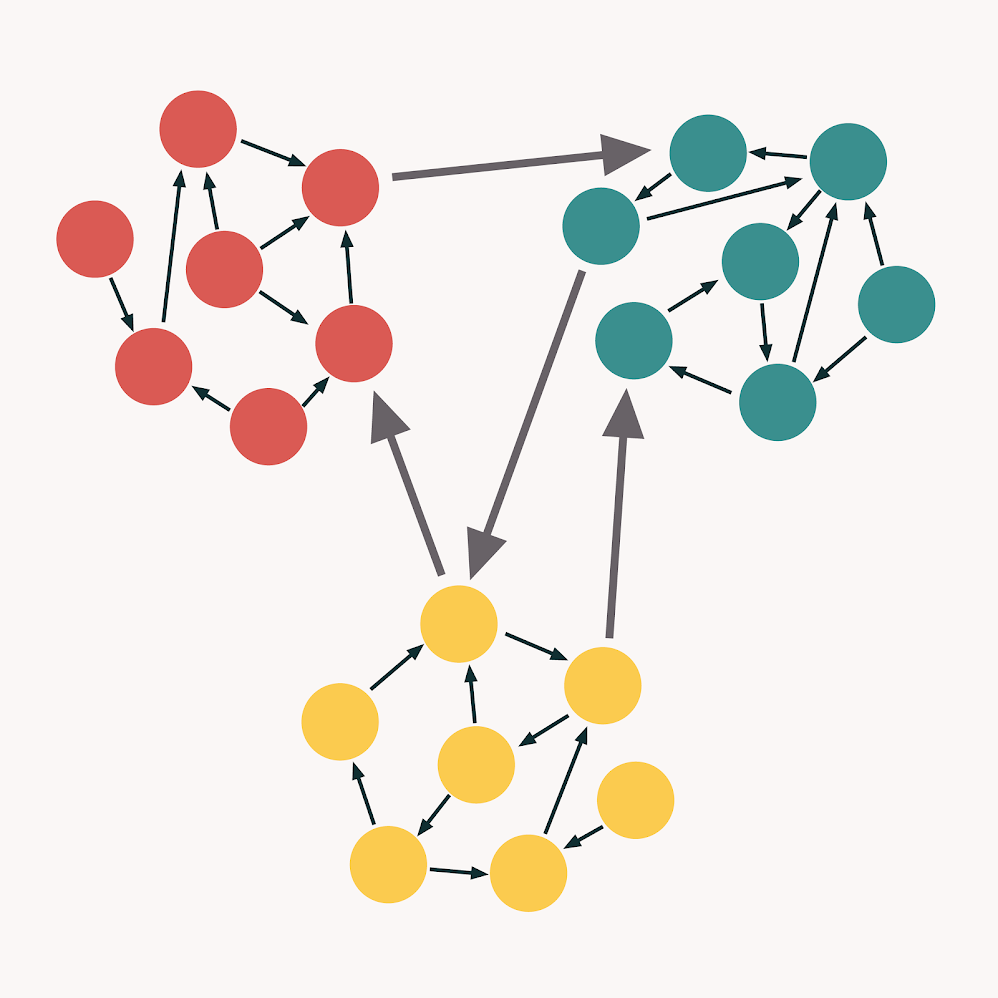
\includegraphics[width=.2\textwidth]{cohesion-2.1.png} \par
\par\columnbreak\par
2. God Object \par
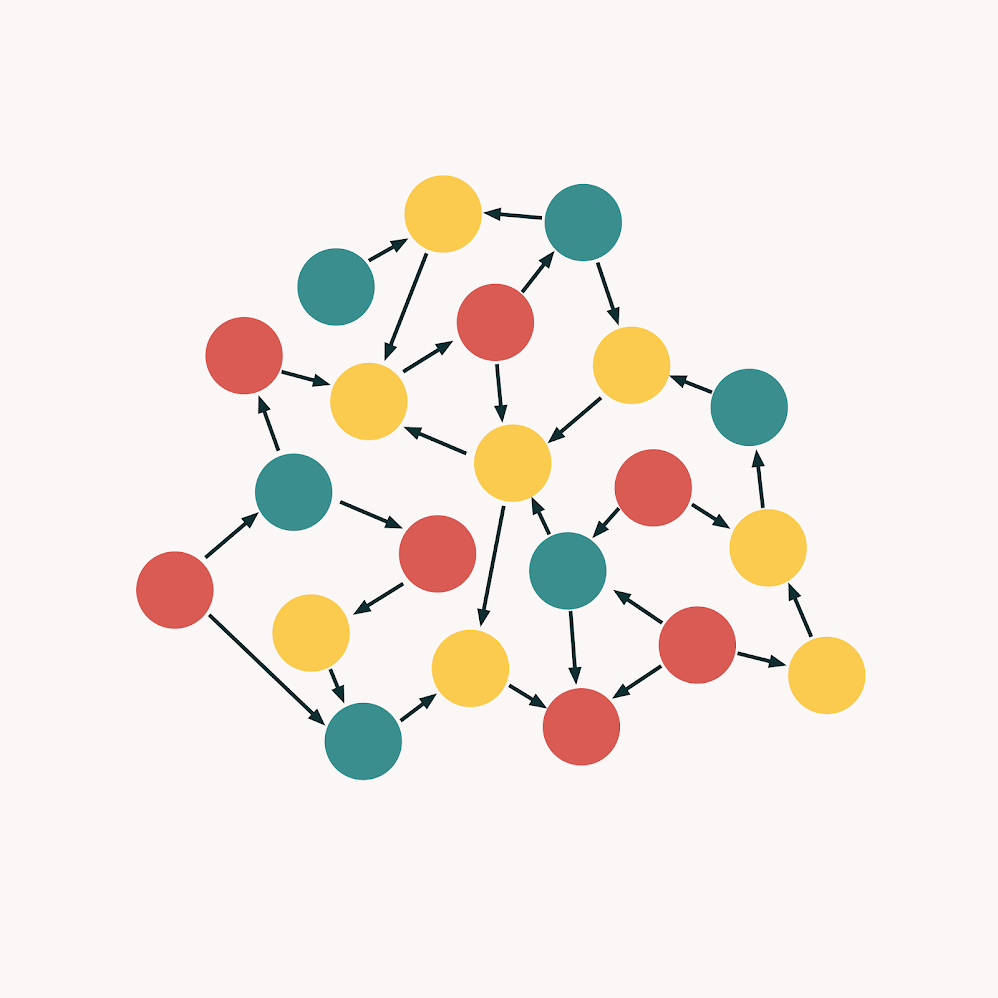
\includegraphics[width=.2\textwidth]{cohesion-2.2.png} \par
\par\columnbreak\par
3. Poorly selected boundaries \par
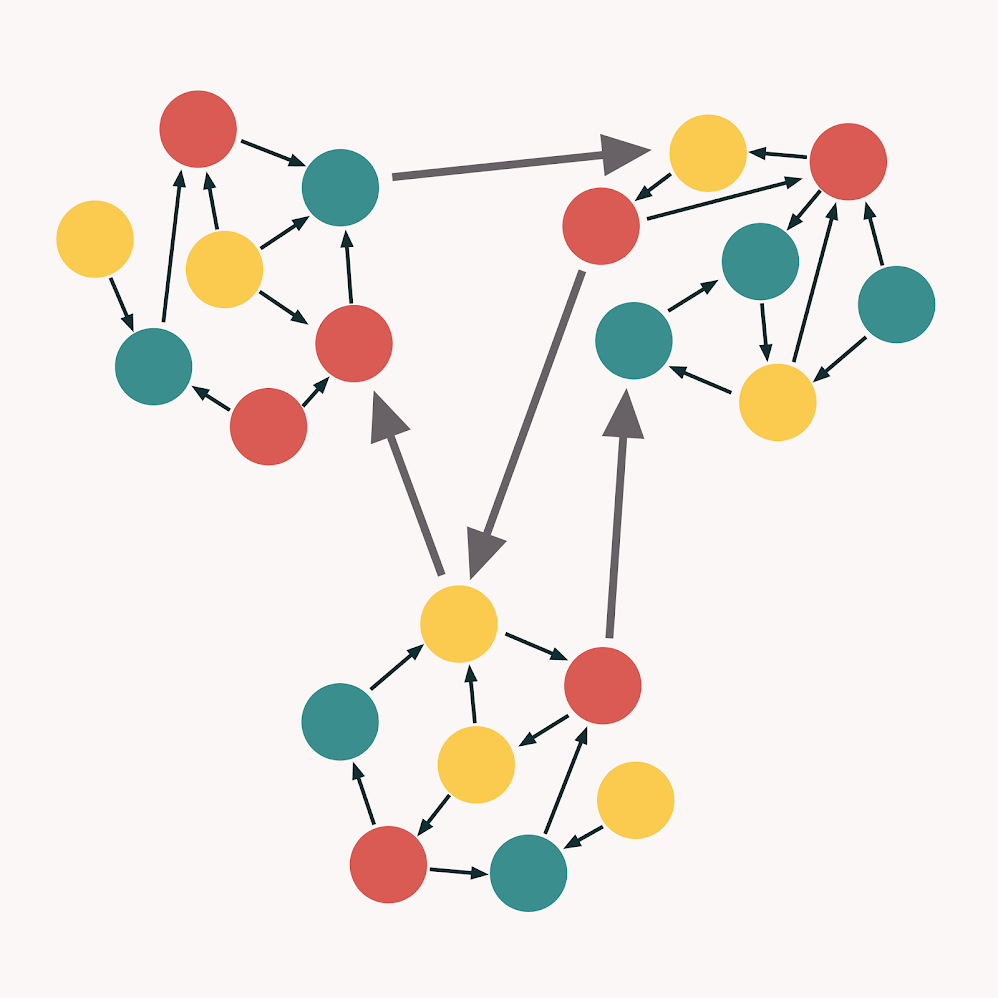
\includegraphics[width=.2\textwidth]{cohesion-2.3.png} \par
\par\columnbreak\par
4. Destructive decoupling \par
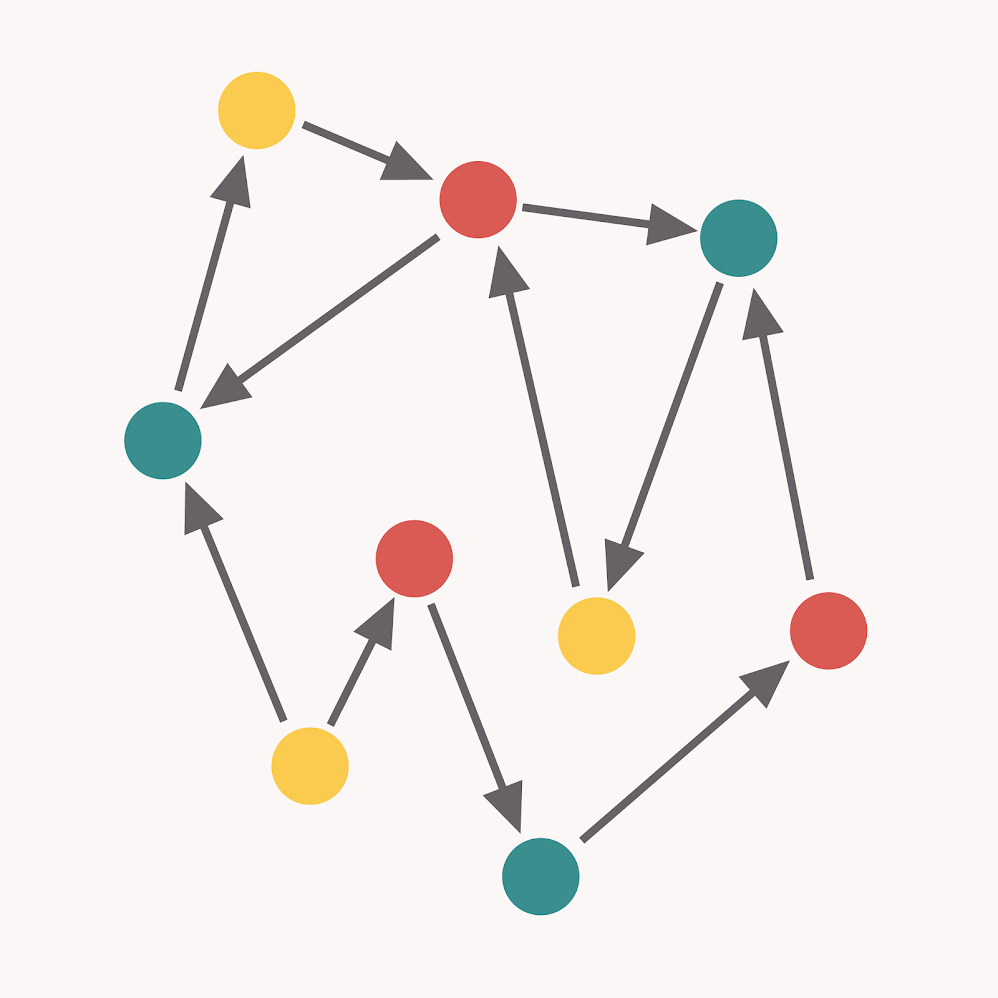
\includegraphics[width=.2\textwidth]{cohesion-2.4.png} \par
\end{multicols}
{\scriptsize Source: \url{https://enterprisecraftsmanship.com/posts/cohesion-coupling-difference/}\par}}

\lnQuote
  [Chris Kemerer]
  {chris-kemerer}
  {Consider a class with methods \(m_1, m_2, \dots, m_n\). Let \(V_i\) be a set of instance variables used by method \(m_i\). There are \(n\) such sets \(V_1, V_2, \dots, V_n\). LCOM is the number of disjoint sets formed by the intersection of the \(n\) sets. The number of disjoint sets provides a measure for the disparate nature of methods in the class. Fewer disjoint sets implies greater similarity of methods.}
  {chidamber1991towards}

\pptBanner{LCOM Example (not working)}
\begin{multicols}{2}
{\small\begin{ffcode}
class Rectangle {
  int x, y, w, h;
  int area() {
    return w * h; }
  int move(int dx, dy) {
    x += dx; y += dy; }
  int resize(int dx, dy) {
    w += dx; h += dy; }
  bool tall() {
    return h > 100; }
}
\end{ffcode}
}
\par\columnbreak\par
\( M = \{ \texttt{area}, \texttt{move}, \texttt{resize}, \texttt{tall} \} \) \par
\( v_\texttt{area} = \{ \texttt{w}, \texttt{h} \} \) \par
\( v_\texttt{move} = \{ \texttt{x}, \texttt{y} \} \) \par
\( v_\texttt{resize} = \{ \texttt{w}, \texttt{h} \} \) \par
\( v_\texttt{tall} = \{ \texttt{h} \} \) \par
LCOM is the number of disjoint sets formed by the intersection of the \(n\) sets. \textcolor{red}{WTF?}
\end{multicols}
\plush{}

\lnQuote
  [Chris F. Kemerer]
  {../07-LCOM/kemerer}
  {Let \(P = \{ (v_i, v_j) | v_i \cap v_j = \emptyset \}\) and \(Q = \{ (v_i, v_j) | v_i \cap v_j \not= \emptyset \}\). Then, \( \texttt{LCOM} = |P| - |Q| \), but not less than zero. Thus, the LCOM is a count of the number of method pairs whose similarity is 0 minus the count of method pairs whose similarity is not zero.}
  {chidamber1994metrics}

\pptBanner{LCOM Example (working)}
\begin{multicols}{2}
{\small\begin{ffcode}
class Rectangle {
  int x, y, w, h;
  int area() {
    return w * h; }
  int move(int dx, dy) {
    x += dx; y += dy; }
  int resize(int dx, dy) {
    w += dx; h += dy; }
  bool tall() {
    return h > 100; }
}
\end{ffcode}
}
\par\columnbreak\par
{\small\( M = \{ \texttt{area}, \texttt{move}, \texttt{resize}, \texttt{tall} \} \) \\
\( v_\texttt{area} = \{ \texttt{w}, \texttt{h} \} \) \\
\( v_\texttt{move} = \{ \texttt{x}, \texttt{y} \} \) \\
\( v_\texttt{resize} = \{ \texttt{w}, \texttt{h} \} \) \\
\( v_\texttt{tall} = \{ \texttt{h} \} \) \par
\( P = \{ (v_\texttt{area}, v_\texttt{move}), \) \\
\( \quad (v_\texttt{move}, v_\texttt{resize}) \} \) \\
\( Q = \{ (v_\texttt{area}, v_\texttt{resize}), \) \\
\( \quad (v_\texttt{area}, v_\texttt{tall}), \) \\
\( \quad (v_\texttt{resize}, v_\texttt{tall}) \} \) \par
\( \texttt{LCOM} = |P| - |Q| = 2 - 3 = -1 \to 0\) \\}
\end{multicols}
\plush{}

\lnQuote
  [Brian Henderson-Sellers]
  {brian-henderson-sellers}
  {LCOM2 equals the percentage of methods that do not access a specific attribute averaged over all attributes in the class. If the number of methods or attributes is zero, LCOM2 is undefined and displayed as zero.}
  {henderson1996coupling}

\pptBanner{LCOM2 Example}
\begin{multicols}{2}
{\small\begin{ffcode}
class Rectangle {
  int x, y, w, h;
  int area() {
    return w * h; }
  int move(int dx, dy) {
    x += dx; y += dy; }
  int resize(int dx, dy) {
    w += dx; h += dy; }
  bool tall() {
    return h > 100; }
}
\end{ffcode}
}
\par\columnbreak\par
\( a_\texttt{x} = 3 / 4 = 0.75 \) \par
\( a_\texttt{y} = 3 / 4 = 0.75 \) \par
\( a_\texttt{w} = 2 / 4 = 0.5 \) \par
\( a_\texttt{h} = 1 / 4 = 0.25 \) \par
\( \texttt{LCOM2} = (0.75 + 0.75 + 0.5 + 0.25) / 4 = 0.5625 \) \par
{\scriptsize Source: \url{https://www.aivosto.com/project/help/pm-oo-cohesion.html}\par}
\end{multicols}
\plush{}

\lnQuote
  [Larry Constantine]
  {larry-constantine}
  {LCOM3 is defined as a normalized measure that considers the number of methods in the class, the number of attributes, and the average number of methods that access each attribute. (by ChatGPT)}
  {henderson1996coupling}

\pptBanner{LCOM3 Example}
\begin{multicols}{2}
{\small\begin{ffcode}
class Rectangle {
  int x, y, w, h;
  int area() {
    return w * h; }
  int move(int dx, dy) {
    x += dx; y += dy; }
  int resize(int dx, dy) {
    w += dx; h += dy; }
  bool tall() {
    return h > 100; }
}
\end{ffcode}
}
\par\columnbreak\par
\(\texttt{LCOM3} = (m - t) / ( m - 1) = 1.1875 \)\par
where\par
\( m = 4 \) (total methods in the class) \par
\( t = 0.4375 \) (how many methods access one var) \par
\end{multicols}
\plush{}

\lnQuote
  [Martin Hitz]
  {martin-hitz}
  {LCOM4 measures the number of 'connected components' in a class. A connected component is a set of related methods (and class-level variables). Methods A and B are related if: they both access the same class-level variable, or A calls B or vice versa.}
  {hitz1995measuring}

\pptBanner{LCOM4 Example}
\begin{multicols}{2}
{\small\begin{ffcode}
class Rectangle {
  int x, y, w, h;
  int area() {
    return w * h; }
  int move(int dx, dy) {
    x += dx; y += dy; }
  int resize(int dx, dy) {
    w += dx; h += dy; }
  bool tall() {
    return h > 100; }
}
\end{ffcode}
}
\par\columnbreak\par
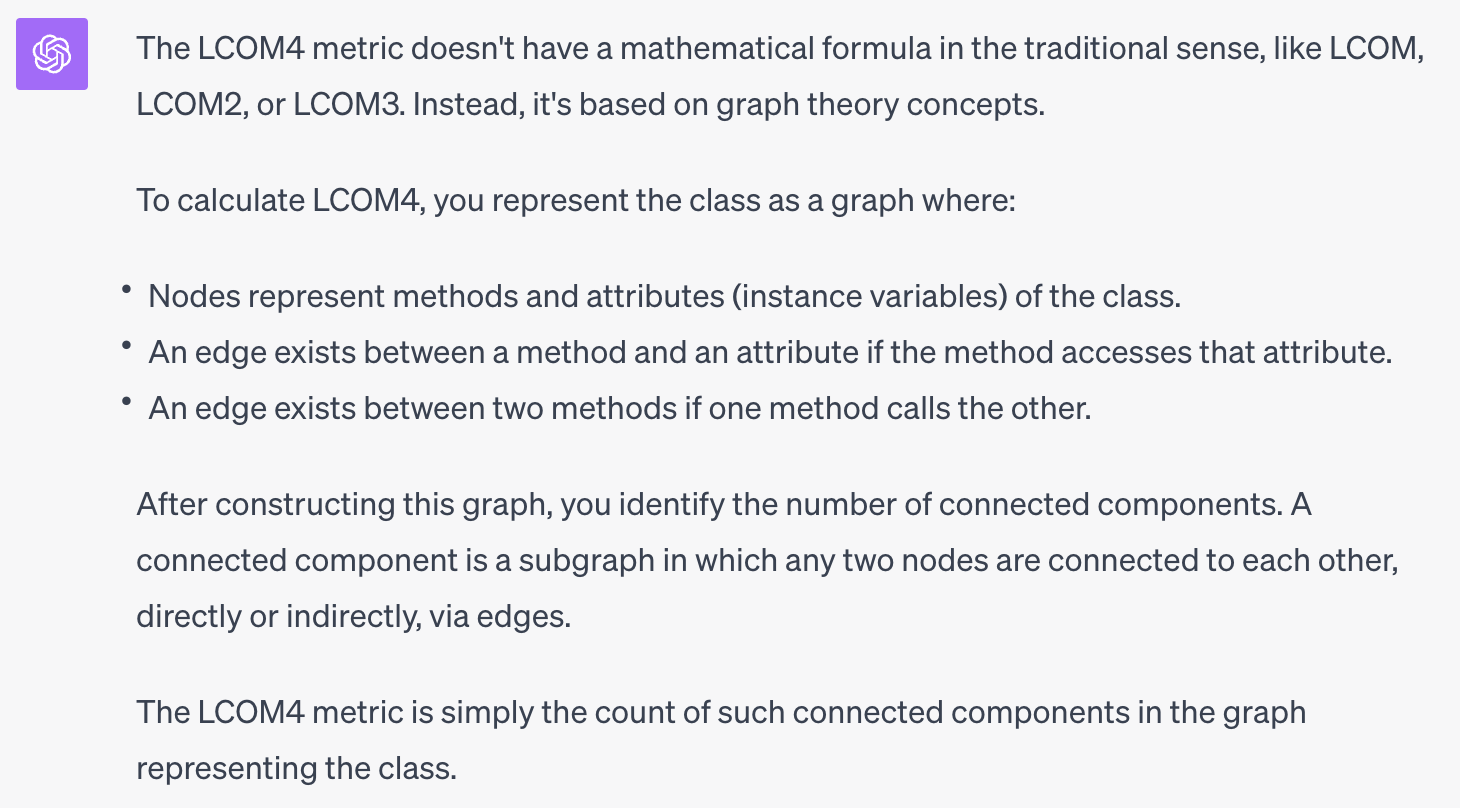
\includegraphics[width=\columnwidth]{lcom4-gpt.png}
\(C_1 = \{ \texttt{x}, \texttt{y}, \texttt{move} \} \)\par
\(C_2 = \{ \texttt{w}, \texttt{h}, \texttt{move}, \texttt{resize}, \texttt{tall} \} \)\par
\(\texttt{LCOM4} = 2 \)\par
\end{multicols}
\plush{}

\lnPitch{LCOMs can be calculated by a few tools:
\begin{itemize}
\item \href{https://www.jpeek.org}{jPeek} for Java
\item \href{https://www.cppdepend.com/documentation/code-metrics}{CPPDepend} for C++
\item \href{https://github.com/FujiHaruka/eslint-plugin-lcom}{eslint-plugin-lcom} for JavaScript
\item \href{https://pypi.org/project/lcom/}{lcom} for Python
\item \href{https://github.com/yahoojapan/lcom4go}{lcom4go} for Go
\end{itemize}}

\lnPitch{
  \pptBanner{jPeek}
  \begin{multicols}{2}
  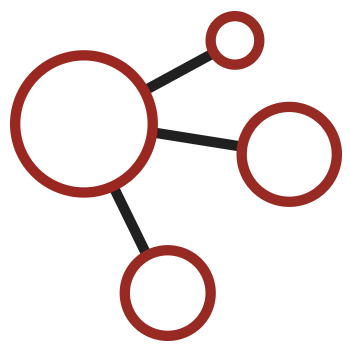
\includegraphics[width=6em]{jpeek-logo.png}\par
  \url{https://www.jpeek.org}
  \par\columnbreak\par
  Motivation: ``Class cohesion is considered as one of most important object-oriented software attributes. There are over 30 different cohesion metrics invented so far, but almost none of them have calculators available. We want to create such a tool that will make it possible to analyze code quality more or less formally.''
  \end{multicols}}

\end{document}
